\subsection{Clamping & Distortion}

/FloatBarrier

\begin{figure}[h!]
	\centering
	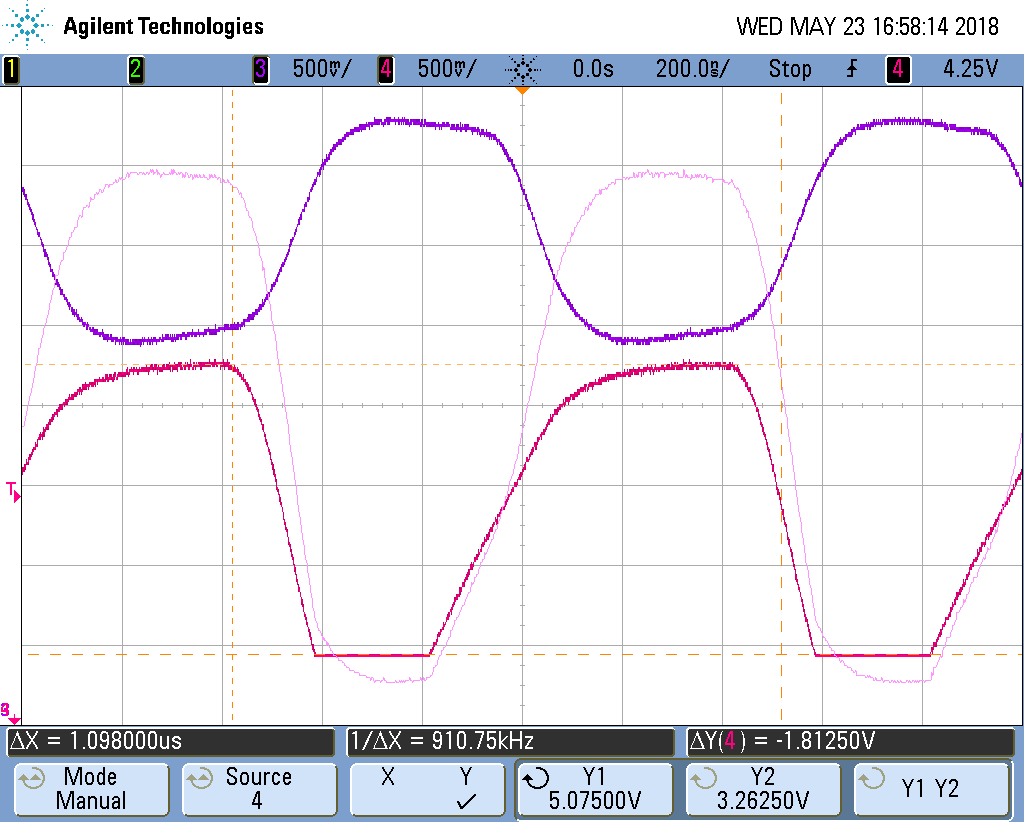
\includegraphics[scale=0.60]{./images/scope_7}
	\caption{Measured maximum signal swing of V_{in-} from a 2\si{\volt} p/p input at 1MHz}
	\label{fig:scope_7}
\end{figure}

\FloatBarrier

\begin{figure}[h!]
	\centering
	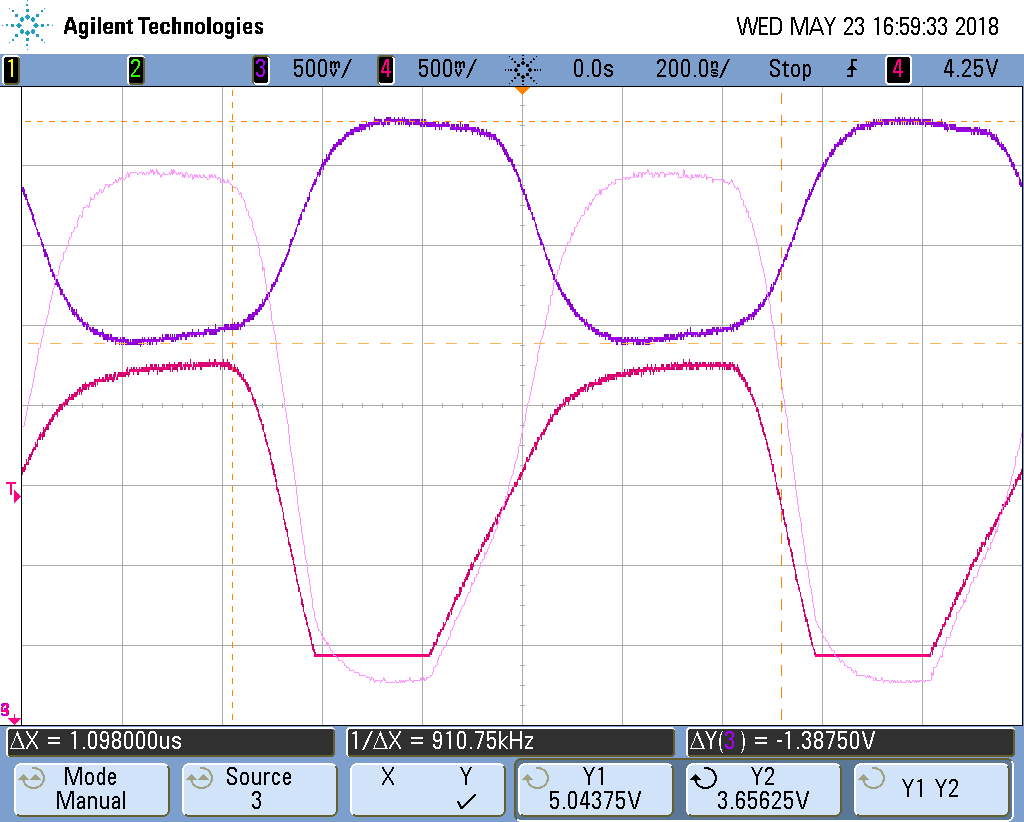
\includegraphics[scale=0.60]{./images/scope_8}
	\caption{Measured maximum signal swing of V_{in+} from a 2\si{\volt} p/p input at 1MHz}
	\label{fig:scope_8}
\end{figure}

\FloatBarrier

From the cursors in (\ref{fig:scope_7}), V_{in-} ranges from 5.075 to 3.262 \si{\volt}, resulting in a swing of 1.81\si{\volt}.
Similarly, the cursors in (\ref{fig:scope_8}) reveal a range of 1.38\si{\volt}.
Thus, the voltage range for the signal V_{out+} - V_{out-} is the sum of these two ranges, or 3.19\si{\volt}.
From these parameters, an input signal that will avoid clipping should be lower than 3.19\si{\volt} / A_{DM} \approx 1.5 \si{\volt}.